\section{Simple Angles}

There is a set of angles around the unit circle, which we refer to as the {\bf simple angles}, due to the simplicity in form of the sine and cosine at these angles.  It will be expected for you to recreate these values on demand in the future, make sure you study them well.\\

\begin{figure}[htb]
\center
\caption{Simple angles in degrees.}
\label{fig:simple_angles_degrees}
\begin{tikzpicture}[inner sep=0pt,minimum size=0mm]

\LLANGLE{0,0}{2}{0}{30}{$30^o$}{0.5}
\LLANGLE{0,0}{2}{30}{45}{$45^o$}{0.5}
\LLANGLE{0,0}{2}{45}{60}{$60^o$}{0.5}
\LLANGLE{0,0}{2}{60}{90}{$90^o$}{0.5}

\LLANGLE{0,0}{2}{90}{120}{$120^o$}{0.5}
\LLANGLE{0,0}{2}{120}{135}{$135^o$}{0.5}
\LLANGLE{0,0}{2}{135}{150}{$150^o$}{0.5}
\LLANGLE{0,0}{2}{150}{180}{$180^o$}{0.5}

\LLANGLE{0,0}{2}{180}{210}{$210^o$}{0.5}
\LLANGLE{0,0}{2}{210}{225}{$225^o$}{0.5}
\LLANGLE{0,0}{2}{225}{240}{$240^o$}{0.5}
\LLANGLE{0,0}{2}{240}{270}{$270^o$}{0.5}

\LLANGLE{0,0}{2}{270}{300}{$300^o$}{0.5}
\LLANGLE{0,0}{2}{300}{315}{$315^o$}{0.5}
\LLANGLE{0,0}{2}{315}{330}{$330^o$}{0.5}
\LLANGLE{0,0}{2}{330}{360}{$0^o, 360^o$}{.75}

\end{tikzpicture}
\end{figure}

\begin{figure}[htb]
\center
\caption{Simple angles in radians.}
\label{fig:simple_angles_radians}
\begin{tikzpicture}[inner sep=0pt,minimum size=0mm]

\LLANGLE{0,0}{2}{0}{30}{$\pisix^c$}{0.5}
\LLANGLE{0,0}{2}{30}{45}{$\pifour^c$}{0.5}
\LLANGLE{0,0}{2}{45}{60}{$\pithree^c$}{0.5}
\LLANGLE{0,0}{2}{60}{90}{$\pitwo^c$}{0.5}

\LLANGLE{0,0}{2}{90}{120}{$\twopithree^c$}{0.5}
\LLANGLE{0,0}{2}{120}{135}{$\threepifour^c$}{0.5}
\LLANGLE{0,0}{2}{135}{150}{$\fivepisix^c$}{0.5}
\LLANGLE{0,0}{2}{150}{180}{$\pi^c$}{0.5}

\LLANGLE{0,0}{2}{180}{210}{$\sevenpisix^c$}{0.5}
\LLANGLE{0,0}{2}{210}{225}{$\fivepifour^c$}{0.5}
\LLANGLE{0,0}{2}{225}{240}{$\fourpithree^c$}{0.5}
\LLANGLE{0,0}{2}{240}{270}{$\threepitwo^c$}{0.5}

\LLANGLE{0,0}{2}{270}{300}{$\fivepithree^c$}{0.5}
\LLANGLE{0,0}{2}{300}{315}{$\sevenpifour^c$}{0.5}
\LLANGLE{0,0}{2}{315}{330}{$\elevenpisix^c$}{0.5}
\LLANGLE{0,0}{2}{330}{360}{$0^c, 2\pi^c$}{0.75}

\end{tikzpicture}
\end{figure}

These figures can be confusing, so we will split the unit circle into quadrants and memorize a piece at a time.\\

\subsection{First Quadrant}

We will start with the simple angles in the first quadrant, or the quarter of our circle where both the x and y projections are $\geq 0$.  The simple angles in the first quadrant are $0$, $\pisix$, $\pifour$, $\pithree$, and $\pitwo$.  Looking at these angles graphically, you can see that $0$ and $\pitwo$ bound the quarter circle in the first quadrant, $\pifour$ splits the quarter circle into halves, and $\pisix$ and $\pifour$ split it into thirds.\\

\begin{figure}[htb]
\center
\caption{Sine and cosine of the first quadrant.}
\label{fig:sine_and_cosine_of_the_first_quadrant}
\begin{tikzpicture}[inner sep=0pt,minimum size=0mm]

\node at (0,7.5) {};

\node[inner sep = 4pt] at (3, -1.25) {$cos$};
\node[inner sep = 4pt] at (-1.25,3) {$sin$};


\node[inner sep = 4pt] at (6.0*1,-0.5) {$1$};
\node[inner sep = 4pt] at (6.0*0.866,-0.5) {$\frac{\sqrt{3}}{2}$};
\node[inner sep = 4pt] at (6.0*0.7071,-0.5) {$\frac{\sqrt{2}}{2}$};
\node[inner sep = 4pt] at (6.0*0.5,-0.5) {$\frac{1}{2}$};
\node[inner sep = 4pt] at (6.0*0.0,-0.5) {$0$};

\node[inner sep = 4pt] at (-0.5,6.0*1) {$1$};
\node[inner sep = 4pt] at (-0.5,6.0*0.866) {$\frac{\sqrt{3}}{2}$};
\node[inner sep = 4pt] at (-0.5,6.0*0.7071) {$\frac{\sqrt{2}}{2}$};
\node[inner sep = 4pt] at (-0.5,6.0*0.5) {$\frac{1}{2}$};
\node[inner sep = 4pt] at (-0.5,6.0*0.0) {$0$};


\LLANGLE{0,0}{6}{0}{0}{$0^o$}{0.5}
\LLANGLE{0,0}{6}{0}{30}{$30^o$}{0.5}
\LLANGLE{0,0}{6}{30}{45}{$45^o$}{0.5}
\LLANGLE{0,0}{6}{45}{60}{$60^o$}{0.5}
\LLANGLE{0,0}{6}{60}{90}{$90^o$}{0.5}

\draw[dashed] (6*0.866,6*0.0) -- (6*0.866,6*0.5);
\draw[dashed] (6*0.70701,6*0.0) -- (6*0.7071,6*0.7071);
\draw[dashed] (6*0.5,6*0.0) -- (6*0.5,6*0.866);

\draw[dashed] (6*0.0,6*0.866) -- (6*0.5,6*0.866);
\draw[dashed] (6*0.0,6*0.7071) -- (6*0.7071,6*0.7071);
\draw[dashed] (6*0.0,6*0.5) -- (6*0.866,6*0.5);

\end{tikzpicture}
\end{figure}

The following table shows the sine and cosine of angles in the first quadrant.  These values are also shown graphically.\\

\begin{figure}[htb]
\caption{Sine and cosine of simple angles in the first quadrant.}
\label{fig:simple_angles_first_quadrant}
\begin{center}
\begin{tabular}{ | c | c | c | c | c | c | }
\hline 
$\theta$ & $0^c , 0^o$ & $\frac{\pi}{6}^c , 30^o$ & $\frac{\pi}{4}^c , 45^o$ & $\frac{\pi}{3}^c , 60^o$ & $\pitwo^c , 90^o$\\
\hline 
$sin(\theta)$ & $\sqrt{\frac{0}{4}}$ & $\sqrt{\frac{1}{4}}$ & $\sqrt{\frac{2}{4}}$ & $\sqrt{\frac{3}{4}}$ & $\sqrt{\frac{4}{4}}$\\
\hline 
$cos(\theta)$ & $\sqrt{\frac{4}{4}}$ & $\sqrt{\frac{3}{4}}$ & $\sqrt{\frac{2}{4}}$ & $\sqrt{\frac{1}{4}}$ & $\sqrt{\frac{0}{4}}$\\
\hline 
$tan(\theta)$ & $\sqrt{\frac{0}{4}}$ & $\sqrt{\frac{1}{3}}$ & $\sqrt{\frac{2}{2}}$ & $\sqrt{\frac{3}{1}}$ & $\sqrt{\frac{4}{0}}$\\
\hline
\end{tabular}
\end{center}
\end{figure}

\newpage

A first useful observation is that sine and cosine have the same values for these angles, but in reverse orders.  A second observation is that all the values of sine and cosine at these angles are the square root of some fraction of fourths.  This is an example of why these angles are useful to memorize; not only are the measures of these angles simple expressions in radians or degrees, but the sine and cosine of these angles are also simple expressions.

\begin{figure}[htb]
\caption{Simplified sine and cosine of the first quadrant.}
\label{fig:simplified_first_quadrant}
\begin{center}
\begin{tabular}{ | c | c | c | c | c | c | }
\hline 
$\theta$ & $0^c , 0^o$ & $\frac{\pi}{6}^c , 30^o$ & $\frac{\pi}{4}^c , 45^o$ & $\frac{\pi}{3}^c , 60^o$ & $\pitwo^c , 90^o$\\
\hline 
$sin(\theta)$ & $0$ & $\frac{1}{2}$ & $\frac{\sqrt{2}}{2}$ & $\frac{\sqrt{3}}{2}$ & $1$\\
\hline 
$cos(\theta)$ & $1$ & $\frac{\sqrt{3}}{2}$ & $\frac{\sqrt{2}}{2}$ & $\frac{1}{2}$ & $0$\\
\hline 
$tan(\theta)$ & $0$ & $\frac{\sqrt{3}}{3}$ & $1$ & $\sqrt{3}$ & $nan$\\
\hline
\end{tabular}
\end{center}
\end{figure}

Another important thing to note is the tangent of $90^o$ has a zero denominator.  The tangent of $90^o$ does not exists, and thus is not a number (nan).  This will be explained in depth later.

\clearpage
\subsection{Second Quadrant}

The simple angles for the second quadrant($x \leq 0 , y \geq 0$) can be found by adding \pitwo to each simple angle in the first quadrant.  This is equivalent to a rotation by a quarter-circle.  As well, this quadrant is a reflection of the first quadrant across the y axis.  Thus, the x projections (cosine) become negative, but the y projections (sine) remain positive.\\

\begin{figure}[htb]
\center
\caption{Sine and cosine of the second quadrant.}
\label{fig:sine_and_cosine_of_the_second_quadrant}
\begin{tikzpicture}[inner sep=0pt,minimum size=0mm]

\node at (0,7.5) {};
\node[inner sep = 4pt] at (-3, -1) {$cos$};
\node[inner sep = 4pt] at (1.25,3) {$sin$};

\node[inner sep = 4pt] at (-6.0*1,-0.5) {$-1$};
\node[inner sep = 4pt] at (-6.0*0.866,-0.5) {$-\frac{\sqrt{3}}{2}$};
\node[inner sep = 4pt] at (-6.0*0.7071,-0.5) {$-\frac{\sqrt{2}}{2}$};
\node[inner sep = 4pt] at (-6.0*0.5,-0.5) {$-\frac{1}{2}$};
\node[inner sep = 4pt] at (-6.0*0.0,-0.5) {$0$};

\node[inner sep = 4pt] at (0.5,6.0*1) {$1$};
\node[inner sep = 4pt] at (0.5,6.0*0.866) {$\frac{\sqrt{3}}{2}$};
\node[inner sep = 4pt] at (0.5,6.0*0.7071) {$\frac{\sqrt{2}}{2}$};
\node[inner sep = 4pt] at (0.5,6.0*0.5) {$\frac{1}{2}$};
\node[inner sep = 4pt] at (0.5,6.0*0.0) {$0$};


\LLANGLE{0,0}{6}{90}{90}{$90^o$}{0.5}
\LLANGLE{0,0}{6}{90}{120}{$120^o$}{0.5}
\LLANGLE{0,0}{6}{120}{135}{$135^o$}{0.5}
\LLANGLE{0,0}{6}{135}{150}{$150^o$}{0.5}
\LLANGLE{0,0}{6}{150}{180}{$180^o$}{0.5}

\draw[dashed] (-6*0.866,6*0.0) -- (-6*0.866,6*0.5);
\draw[dashed] (-6*0.70701,6*0.0) -- (-6*0.7071,6*0.7071);
\draw[dashed] (-6*0.5,6*0.0) -- (-6*0.5,6*0.866);

\draw[dashed] (-6*0.0,6*0.866) -- (-6*0.5,6*0.866);
\draw[dashed] (-6*0.0,6*0.7071) -- (-6*0.7071,6*0.7071);
\draw[dashed] (-6*0.0,6*0.5) -- (-6*0.866,6*0.5);

\end{tikzpicture}

\begin{center}
\begin{tabular}{ | c | c | c | c | c | c | }
\hline 
$\theta$ & $\pitwo$ & $\fivepisix$ & $\threepifour$ & $\fivepisix$ & $\pi$\\
\hline 
$sin(\theta)$ & $\sqrt{\frac{4}{4}}$ & $\sqrt{\frac{3}{4}}$ & $\sqrt{\frac{2}{4}}$ & $\sqrt{\frac{1}{4}}$ & $\sqrt{\frac{0}{4}}$\\
\hline 
$cos(\theta)$ & $-\sqrt{\frac{0}{4}}$ & $-\sqrt{\frac{1}{4}}$ & $-\sqrt{\frac{2}{4}}$ & $-\sqrt{\frac{3}{4}}$ & $-\sqrt{\frac{4}{4}}$\\
\hline 
$tan(\theta)$ & $-\sqrt{\frac{4}{0}}$ & $-\sqrt{\frac{3}{1}}$ & $-\sqrt{\frac{2}{2}}$ & $-\sqrt{\frac{1}{3}}$ & $-\sqrt{\frac{0}{4}}$\\
\hline
\end{tabular}
\end{center}
\end{figure}

\clearpage
\subsection{Third Quadrant}

The simple angles in the third qudrant are $\pi$, $\sevenpisix$, $\fivepifour$, $\fourpithree$, and $\threepitwo$.  An additional reflection across the x axis implies that both x and y projections will be negated.\\

\begin{figure}[htb]
\center
\caption{Sine and cosine of the third quadrant.}
\label{fig:sine_and_cosine_of_the_third_quadrant}
\begin{tikzpicture}[inner sep=0pt,minimum size=0mm]

\node at (0,1.5) {};
\node[inner sep = 4pt] at (-3, 1) {$cos$};
\node[inner sep = 4pt] at (1.25,-3) {$sin$};

\node[inner sep = 4pt] at (-6.0*1,0.5) {$-1$};
\node[inner sep = 4pt] at (-6.0*0.866,0.5) {$-\frac{\sqrt{3}}{2}$};
\node[inner sep = 4pt] at (-6.0*0.7071,0.5) {$-\frac{\sqrt{2}}{2}$};
\node[inner sep = 4pt] at (-6.0*0.5,0.5) {$-\frac{1}{2}$};
\node[inner sep = 4pt] at (-6.0*0.0,0.5) {$0$};

\node[inner sep = 4pt] at (0.5,-6.0*1) {$-1$};
\node[inner sep = 4pt] at (0.5,-6.0*0.866) {$-\frac{\sqrt{3}}{2}$};
\node[inner sep = 4pt] at (0.5,-6.0*0.7071) {$-\frac{\sqrt{2}}{2}$};
\node[inner sep = 4pt] at (0.5,-6.0*0.5) {$-\frac{1}{2}$};
\node[inner sep = 4pt] at (0.5,-6.0*0.0) {$0$};


\LLANGLE{0,0}{6}{180}{180}{$180^o$}{0.5}
\LLANGLE{0,0}{6}{180}{210}{$210^o$}{0.5}
\LLANGLE{0,0}{6}{210}{225}{$225^o$}{0.5}
\LLANGLE{0,0}{6}{225}{240}{$240^o$}{0.5}
\LLANGLE{0,0}{6}{240}{270}{$270^o$}{0.5}

\draw[dashed] (-6*0.866,-6*0.0) -- (-6*0.866,-6*0.5);
\draw[dashed] (-6*0.70701,-6*0.0) -- (-6*0.7071,-6*0.7071);
\draw[dashed] (-6*0.5,-6*0.0) -- (-6*0.5,-6*0.866);

\draw[dashed] (-6*0.0,-6*0.866) -- (-6*0.5,-6*0.866);
\draw[dashed] (-6*0.0,-6*0.7071) -- (-6*0.7071,-6*0.7071);
\draw[dashed] (-6*0.0,-6*0.5) -- (-6*0.866,-6*0.5);

\end{tikzpicture}

\begin{center}
\begin{tabular}{ | c | c | c | c | c | c | }
\hline 
$\theta$ & $\pi$ & $\sevenpisix$ & $\fivepifour$ & $\fourpithree$ & $\threepitwo$\\
\hline 
$sin(\theta)$ & $-\sqrt{\frac{0}{4}}$ & $-\sqrt{\frac{1}{4}}$ & $-\sqrt{\frac{2}{4}}$ & $-\sqrt{\frac{3}{4}}$ & $-\sqrt{\frac{4}{4}}$\\
\hline 
$cos(\theta)$ & $-\sqrt{\frac{4}{4}}$ & $-\sqrt{\frac{3}{4}}$ & $-\sqrt{\frac{2}{4}}$ & $-\sqrt{\frac{1}{4}}$ & $-\sqrt{\frac{0}{4}}$\\
\hline 
$tan(\theta)$ & $\sqrt{\frac{0}{4}}$ & $\sqrt{\frac{1}{3}}$ & $\sqrt{\frac{2}{2}}$ & $\sqrt{\frac{3}{1}}$ & $\sqrt{\frac{4}{0}}$\\
\hline
\end{tabular}
\end{center}
\end{figure}


\clearpage
\subsection{Fourth Quadrant}
The simple angles in the fourth qudrant are $\threepitwo$, $\fivepithree$, $\sevenpifour$, $\elevenpisix$, and $2\pi$.  This quadrant is equivalent to the reflection of the first quadrant across the x axis, and so the y projections (sine) will be negative, but the x projections (cosine) will be positive. 

\begin{figure}[htb]
\center
\caption{Sine and cosine of the fourth quadrant.}
\label{fig:sine_and_cosine_of_the_fourth_quadrant}
\begin{tikzpicture}[inner sep=0pt,minimum size=0mm]

\node at (0,1.5) {};
\node[inner sep = 4pt] at (3, 1) {$cos$};
\node[inner sep = 4pt] at (-1.25,-3) {$sin$};

\node[inner sep = 4pt] at (6.0*1,0.5) {$1$};
\node[inner sep = 4pt] at (6.0*0.866,0.5) {$\frac{\sqrt{3}}{2}$};
\node[inner sep = 4pt] at (6.0*0.7071,0.5) {$\frac{\sqrt{2}}{2}$};
\node[inner sep = 4pt] at (6.0*0.5,0.5) {$\frac{1}{2}$};
\node[inner sep = 4pt] at (6.0*0.0,0.5) {$0$};

\node[inner sep = 4pt] at (-0.5,-6.0*1) {$-1$};
\node[inner sep = 4pt] at (-0.5,-6.0*0.866) {$-\frac{\sqrt{3}}{2}$};
\node[inner sep = 4pt] at (-0.5,-6.0*0.7071) {$-\frac{\sqrt{2}}{2}$};
\node[inner sep = 4pt] at (-0.5,-6.0*0.5) {$-\frac{1}{2}$};
\node[inner sep = 4pt] at (-0.5,-6.0*0.0) {$0$};

\LLANGLE{0,0}{6}{270}{270}{$270^o$}{0.5}
\LLANGLE{0,0}{6}{270}{300}{$300^o$}{0.5}
\LLANGLE{0,0}{6}{300}{315}{$315^o$}{0.5}
\LLANGLE{0,0}{6}{315}{330}{$330^o$}{0.5}
\LLANGLE{0,0}{6}{330}{360}{$360^o$}{0.5}

\draw[dashed] (6*0.866,-6*0.0) -- (6*0.866,-6*0.5);
\draw[dashed] (6*0.70701,-6*0.0) -- (6*0.7071,-6*0.7071);
\draw[dashed] (6*0.5,-6*0.0) -- (6*0.5,-6*0.866);

\draw[dashed] (6*0.0,-6*0.866) -- (6*0.5,-6*0.866);
\draw[dashed] (6*0.0,-6*0.7071) -- (6*0.7071,-6*0.7071);
\draw[dashed] (6*0.0,-6*0.5) -- (6*0.866,-6*0.5);

\end{tikzpicture}

\begin{center}
\begin{tabular}{ | c | c | c | c | c | c | }
\hline 
$\theta$ & $\threepitwo$ & $\fivepithree$ & $\sevenpifour$ & $\elevenpisix$ & $2\pi$\\
\hline 
$sin(\theta)$ & $-\sqrt{\frac{4}{4}}$ & $-\sqrt{\frac{3}{4}}$ & $-\sqrt{\frac{2}{4}}$ & $-\sqrt{\frac{1}{4}}$ & $-\sqrt{\frac{0}{4}}$\\
\hline 
$cos(\theta)$ & $\sqrt{\frac{0}{4}}$ & $\sqrt{\frac{1}{4}}$ & $\sqrt{\frac{2}{4}}$ & $\sqrt{\frac{3}{4}}$ & $\sqrt{\frac{4}{4}}$\\
\hline 
$tan(\theta)$ & $-\sqrt{\frac{4}{0}}$ & $-\sqrt{\frac{3}{1}}$ & $-\sqrt{\frac{2}{2}}$ & $-\sqrt{\frac{1}{3}}$ & $-\sqrt{\frac{0}{4}}$\\
\hline

\end{tabular}
\end{center}
\end{figure}

\clearpage
\subsection{Review}

Practice drawing this chart, and filling in the angles.  For every angle, write the value in degrees, in radians, and the sine, cosine, and tangent.  You should be able to draw and fill out the entire chart in under five minutes.\\

\begin{figure}[htb]
\center
\caption{Review of simple angles.}
\label{fig:review of simple angles}
\begin{tikzpicture}[inner sep=0pt,minimum size=0mm]

\node at (0,6) {};

\LLANGLE{0,0}{4}{0}{30}{}{0.5}
\LLANGLE{0,0}{4}{30}{45}{}{0.5}
\LLANGLE{0,0}{4}{45}{60}{}{0.5}
\LLANGLE{0,0}{4}{60}{90}{}{0.5}

\LLANGLE{0,0}{4}{90}{120}{}{0.5}
\LLANGLE{0,0}{4}{120}{135}{}{0.5}
\LLANGLE{0,0}{4}{135}{150}{}{0.5}
\LLANGLE{0,0}{4}{150}{180}{}{0.5}

\LLANGLE{0,0}{4}{180}{210}{}{0.5}
\LLANGLE{0,0}{4}{210}{225}{}{0.5}
\LLANGLE{0,0}{4}{225}{240}{}{0.5}
\LLANGLE{0,0}{4}{240}{270}{}{0.5}

\LLANGLE{0,0}{4}{270}{300}{}{0.5}
\LLANGLE{0,0}{4}{300}{315}{}{0.5}
\LLANGLE{0,0}{4}{315}{330}{}{0.5}
\LLANGLE{0,0}{4}{330}{360}{}{.5}

\end{tikzpicture}
\end{figure}

